%% ----------------------------------------------------------------
%% Thesis.tex -- MAIN FILE (the one that you compile with LaTeX)
%% ---------------------------------------------------------------- 

% Set up the document
\documentclass[a4paper, 11pt, oneside]{Thesis}  % Use the "Thesis" style, based on the ECS Thesis style by Steve Gunn

% Include any extra LaTeX packages required
\usepackage[square, numbers, comma, sort&compress]{natbib}  % Use the "Natbib" style for the references in the Bibliography
\usepackage[nottoc]{tocbibind} % bind bibliography to the table of contents
\usepackage{verbatim}  % Needed for the "comment" environment to make LaTeX comments
\usepackage{vector}  % Allows "\bvec{}" and "\buvec{}" for "blackboard" style bold vectors in maths
\usepackage[table]{xcolor}
\hypersetup{urlcolor=black, colorlinks=true}  % Colours hyperlinks in black, can be distracting if there are many links and colored blue.
\usepackage{graphicx}
\graphicspath{{Figures/}}  % Location of the graphics files (set up for graphics to be in PDF format)

%% ----------------------------------------------------------------
\begin{document}
\frontmatter      % Begin Roman style (i, ii, iii, iv...) page numbering

% Set up the Title Page
\title  {DynamiCrypt}
\authors  {Artiom Sumigora}
            
\addresses  {\groupname\\\deptname\\\univname}  % Do not change this here, instead these must be set in the "Thesis.cls" file, please look through it instead
\date       {\today}
\subject    {}
\keywords   {}

\maketitle
%% ----------------------------------------------------------------

\setstretch{1.3}  % It is better to have smaller font and larger line spacing than the other way round

% Define the page headers using the FancyHdr package and set up for one-sided printing
\fancyhead{}  % Clears all page headers and footers
\rhead{\thepage}  % Sets the right side header to show the page number
\lhead{}  % Clears the left side page header

\pagestyle{fancy}  % Finally, use the "fancy" page style to implement the FancyHdr headers

%% ----------------------------------------------------------------
% Declaration Page required for the Thesis
\Declaration{

\addtocontents{toc}{\vspace{1em}}  % Add a gap in the Contents, for aesthetics

I, Artiom Sumigora, declare that this thesis titled, `DynamiCrypt' and the work presented in it are my own. I confirm that:

\begin{itemize} 
\item[\tiny{$\blacksquare$}] This work was done wholly or mainly while in candidature for an undergraduate degree at Cork Institute of Technology.
 
\item[\tiny{$\blacksquare$}] Where any part of this thesis has previously been submitted for a degree or any other qualification at Cork Institute of Technology or any other institution, this has been clearly stated.
 
\item[\tiny{$\blacksquare$}] Where I have consulted the published work of others, this is always clearly attributed.
 
\item[\tiny{$\blacksquare$}] Where I have quoted from the work of others, the source is always given. With the exception of such quotations, this project report is entirely my own work.
 
\item[\tiny{$\blacksquare$}] I have acknowledged all main sources of help.
 
\item[\tiny{$\blacksquare$}] Where the thesis is based on work done by myself jointly with others, I have made clear exactly what was done by others and what I have contributed myself.
\\
\end{itemize}
 
 
Signed:\\
\rule[1em]{25em}{0.5pt}  % This prints a line for the signature
 
Date:\\
\rule[1em]{25em}{0.5pt}  % This prints a line to write the date
}
\clearpage  % Declaration ended, now start a new page

%% ----------------------------------------------------------------

% The Abstract Page
\addtotoc{Abstract}  % Add the "Abstract" page entry to the Contents
\abstract{
\addtocontents{toc}{\vspace{1em}}  % Add a gap in the Contents, for aesthetics

In today's world information is mostly sent in an encrypted form over the public internet. Traditionally when a client connects to a server the public keys are shared and the same set of public/private key pairs are used for the session and potentially for future sessions, depending on how the system is setup. Provided that industry standard encryption is used it would take the attacker longer than the lifetime of the earth to crack the key making the system secure. The problem arises if the attacker managed to get the key in some other fashion other than brute force and got access to the server it would be possible to locate this key and use it to decrypt potentially sensitive information that was captured over the network.

The problem this project proposes to address is that scenario. This will be addressed by using multiple encryption keys throughout the session. These encryption keys will be generated using a tree parity machine. A tree parity machine consists of input neurons, hidden neurons and one output neuron. A neural network is chosen for this because the weights of neural networks can be synchronised between each tree parity machine on different hosts. The weights can then be used to generate a key and since the weights on both tree parity machines are identical the same key will be generated. The weight are synchronised over the network with no information sent about the weights itself therefore the attacker will not be able to figure out the key. The server can then use multiple tree parity machines to synchronise with the same number of tree parity machines on a different server and thus multiple keys will be generated and different keys can be used through a session.

This thesis will provide a program that is capable of handling synchronisation between multiple tree parity machines between two hosts. An API will be provided that will access the said program and allow other server to use dynamic encryption. A NodeJS module will also be provided to make integration with NodeJS applications very easy.

}

\clearpage  % Abstract ended, start a new page
%% ----------------------------------------------------------------

\setstretch{1.3}  % Reset the line-spacing to 1.3 for body text (if it has changed)

% The Acknowledgements page, for thanking everyone
\acknowledgements{
\addtocontents{toc}{\vspace{1em}}  % Add a gap in the Contents, for aesthetics
This project has taken a substantial amount of work, dedication and research. I would
like to say special thanks to:

Dr. John Creagh, project supervisor in semester one.

}
\clearpage  % End of the Acknowledgements
%% ----------------------------------------------------------------

\pagestyle{fancy}  %The page style headers have been "empty" all this time, now use the "fancy" headers as defined before to bring them back


%% ----------------------------------------------------------------
\lhead{\emph{Contents}}  % Set the left side page header to "Contents"
\tableofcontents  % Write out the Table of Contents

%% ----------------------------------------------------------------
\lhead{\emph{List of Figures}}  % Set the left side page header to "List if Figures"
\listoffigures  % Write out the List of Figures

%% ----------------------------------------------------------------
\lhead{\emph{List of Tables}}  % Set the left side page header to "List of Tables"
\listoftables  % Write out the List of Tables

%% ----------------------------------------------------------------
\setstretch{1.5}  % Set the line spacing to 1.5, this makes the following tables easier to read
\clearpage  % Start a new page
\lhead{\emph{Abbreviations}}  % Set the left side page header to "Abbreviations"
\listofsymbols{ll}  % Include a list of Abbreviations (a table of two columns)
{
% \textbf{Acronym} & \textbf{W}hat (it) \textbf{S}tands \textbf{F}or \\
\textbf{TPM} & \textbf{T}ree \textbf{P}arity \textbf{M}achine \\
\textbf{API} & \textbf{A}pplication \textbf{P}rotocol \textbf{I}nterface \\
\textbf{HTTP} & \textbf{H}yper \textbf{T}ext \textbf{T}ransfer \textbf{P}rotocol \\
\textbf{HTTPS} & \textbf{H}yper \textbf{T}ext \textbf{T}ransfer \textbf{P}rotocol \textbf{S}ecure \\
\textbf{SSL} & \textbf{S}ecure \textbf{S}ockets \textbf{L}ayer \\
\textbf{TLS} & \textbf{T}ransfer \textbf{L}ayer \textbf{S}ecurity \\
\textbf{AES} & \textbf{A}dvanced \textbf{E}ncryption \textbf{S}tandard \\
\textbf{RSA} & \textbf{R}ivest \textbf{S}hamir \textbf{A}dleman \\
\textbf{SSH} & \textbf{S}ecure \textbf{S}\textbf{H}ell \\
\textbf{GPG} & \textbf{G}NU \textbf{P}rivacy \textbf{G}uard \\
\textbf{GNU} & \textbf{G}\textbf{N}\textbf{U}'s Not Unix \\
\textbf{AI} & \textbf{A}rtificial \textbf{I}ntelligence \\
\textbf{GAN} & \textbf{G}enerative \textbf{A}dversarial \textbf{N}etwork \\
\textbf{IP} & \textbf{I}nternet \textbf{P}rotocol \\
\textbf{IBM} & \textbf{I}nternational \textbf{B}usiness \textbf{M}achines \\
\textbf{ID} & \textbf{I}\textbf{D}entification \\
\textbf{PHP} & \textbf{H}ypertext \textbf{P}re\textbf{P}rocessor \\
\textbf{KiB} & \textbf{K}\textbf{i}bi\textbf{B}yte \\
\textbf{TCP} & \textbf{T}ransmission \textbf{C}ontrol \textbf{P}rotocol \\
}

%% ----------------------------------------------------------------
% End of the pre-able, contents and lists of things
% Begin the Dedication page

\setstretch{1.3}  % Return the line spacing back to 1.3

\pagestyle{empty}  % Page style needs to be empty for this page
\dedicatory{Dedicated to my family\ldots}

\addtocontents{toc}{\vspace{2em}}  % Add a gap in the Contents, for aesthetics

%% ----------------------------------------------------------------
\mainmatter	  % Begin normal, numeric (1,2,3...) page numbering
\pagestyle{fancy}  % Return the page headers back to the "fancy" style

\chapter{Introduction}
\label{chap:intro}
\lhead{\emph{Introduction}}
This chapter should comprise around 1000 words and introduces your project. Here you are setting the scene, remember the reader may know nothing about your project at this stage (other than the abstract). N.B. The sections outlined in this document are suggested, some projects will have a greater or lesser emphasis on different sections or may change titles and some will have to add other sections to provide context or detail.
% Putting in comments within the TeX file can be really useful in making notes for yourself and dumping text that you intend to edit later

\section{Motivation}
Why is it important to do a project on this topic? This should cover your key motivation for this. For example an excellent student from 2016 noticed a large number of homeless sleeping rough in Cork and was motivated to develop a system that load balanced the homeless shelters to try to accommodate the maximum number of homeless. This section can include the personal pronoun but the rest of the report should be third person passive, this is the case with most technical reports! For example here it is fine to say "... I decided to develop and app to help ...".

\section{Contribution}
Enumerate the main contributions. Here try to zoom out, to talk from the perspective of a Computer Science graduate. In other words, imagine you are talking to a job panel, and you want to show your computer science skills by enumerating how they are reflected in your project work. A good guide here is to look back over the modules you have covered as an undergrad from 2/3rd year, how many tools and techniques from these modules do you have in the project and to what extent? How have you advanced beyond the module content? Do you have anything new?

\section{Structure of This Document}
% notice how I cross referenced the chapters through using the \label tag --> LaTeX is VERY similar to HTML and other mark up languages so you should see nothing new here!
This section is quite formulaic. Briefly describe the structure of this document, enumerating what does each chapter and section stands for. For instance in this work in Chapter \ref{chap:background} the guidance in structuring the literature review is given. Chapter \ref{chap:problem} describes the main requirements for the problem definition and so on ... % Introduction

\chapter{Background}
\label{chap:background}
\lhead{\emph{Background}}
%
%
% Notes Start
%
%
The key question to answer in this chapter is: "What has been done/is being done". 

This chapter comprises around 4000 words and should put your project into context within Computer Science. Your focus here should be on the final section "Current State of the Art". This should be at least 2500 of the 4000 words of this section.
%
%
% Notes End
%
%
\section{Thematic Area within Computer Science}
The Core topic of this project is safely and dynamically encrypting messages between two parties. The communication will rely on multiple functioning NodeJs servers for transfer of encrypted messages. 

The core areas under which my project falls under is cryptography, security for encrypting and securing information. Machine learning will be used for establishing methods of secure information exchange. And finally networking due to the setup required of communicating between different servers and sending encrypted information.


Encryption \cite{encryptionDefinition} is when the plaintext of any form of data that can be easily read is converted to an unreadable encoded version. In order to retrieve the original data for viewing or processing it must be decoded using a specific algorithm and more than likely some sort of key, usually a lengthy password. Encryption may be used for encrypting files and operating systems on a user's hard drive. In today's world encryption is used religiously for data transferred between networks. Sensitive information like user's credentials are constantly being sent from the browser to the server when logging into websites for personalised content. The same is true for for even more high risk information like banking details, scans of identification documents and even keys. Websites that wish to be secure are now using HTTPS instead of HTTP. The Number of websites using HTTPS is constantly increasing see figure \ref{fig:httpsRise}

\begin{figure}[ht]
  \centering
      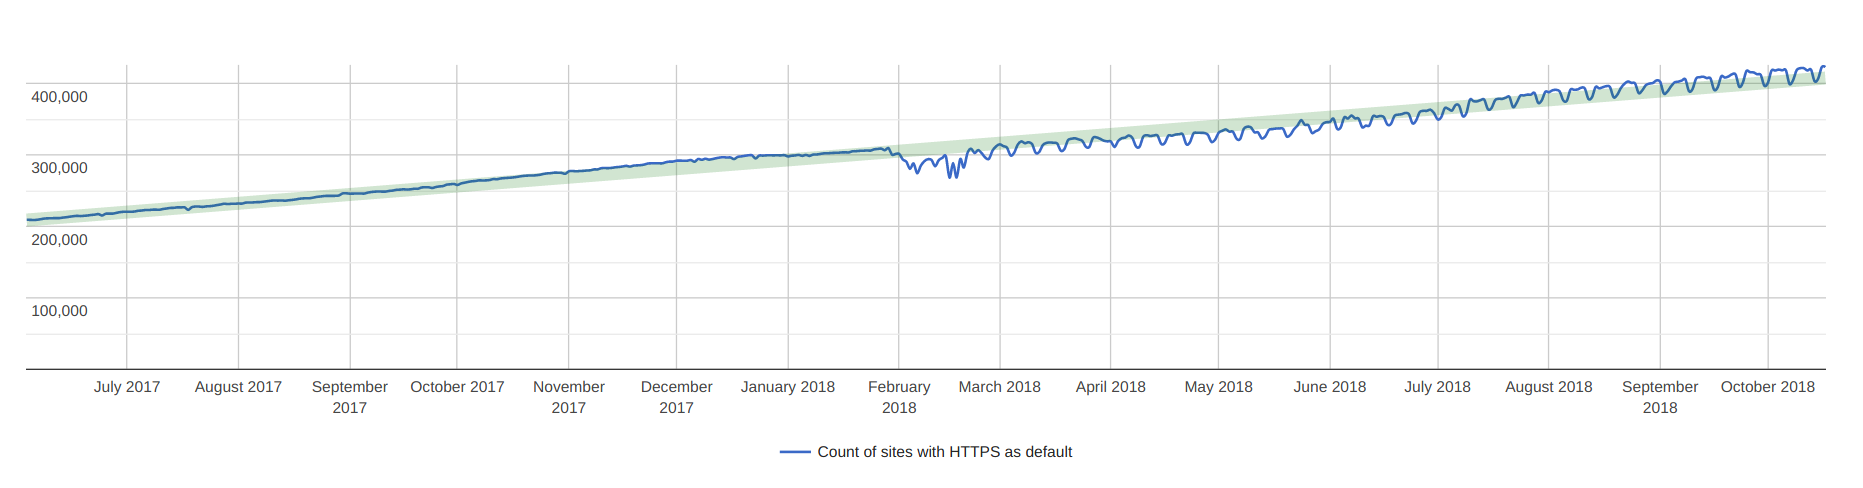
\includegraphics[width=0.9\textwidth]{Figures/httpsRise.png}
  \caption[A graph of HTTPS usage increase]{A graph of HTTPS usage increase\cite{https}}
  \label{fig:httpsRise}
\end{figure}

HTTP is not secure because information transmitted is in plaintext by default and extra steps are needed to encrypt the data. Because the author of the server can choose how the data is encrypted, it can lead to the theft of data as the implementation may not be correct or a weak algorithm is used.
On the other hand if a website uses HTTPS which is a common defined standard there will be minimal data theft see figure \ref{fig:https1}. HTTPS uses SSL or TLS which are protocols that use asymmetric keys (will be discussed later). SSL is generally used more often as it requires the server to acquire an SSL certificate from a trusted third party.

\begin{figure}[ht]
  \centering
      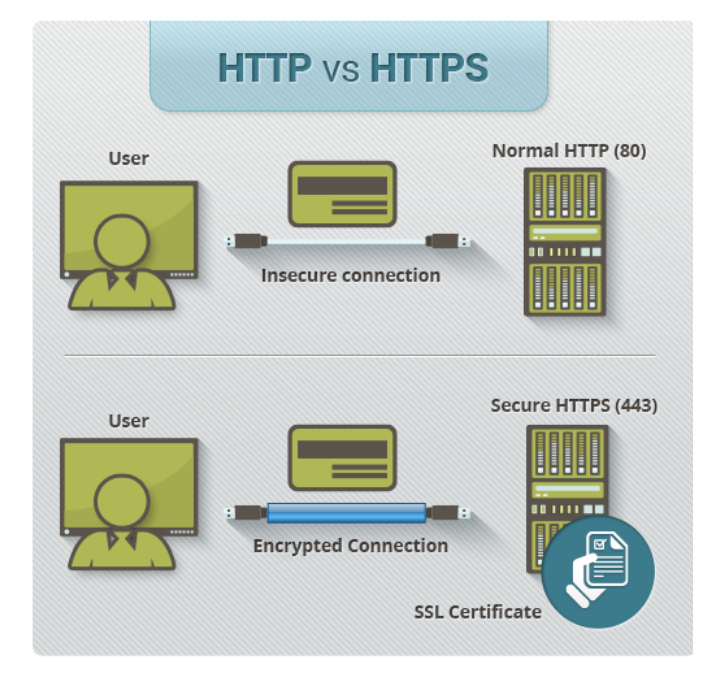
\includegraphics[width=0.6\textwidth]{Figures/httpsVsHttp.png}
  \caption[HTTP vs HTTPS]{HTTP vs HTTPS\cite{https1}}
  \label{fig:https1}
\end{figure}



Traditionally there are two encryption types.
\begin{enumerate}
    \item Symmetric
    \item Asymmetric
\end{enumerate}

Symmetric encryption uses the same key to encrypt and decrypt information. This type of encryption is usually used to encrypt information provided by a human generated key. It is not safe to send this key over a network as it can be stolen or the destination being sent to can be spoofed. There are multiple implementations of symmetric ciphers, the most common being AES, Twofish and Serpent. To increase your security at the cost of encryption and decryption time you can chain multiple ciphers together AES(Twofish(Key)).

Asymmetric or commonly known as public key encryption methods are commonly used for sharing data between between computers on different networks. This is because a set of keys are generated one being private and the other public. The private key is never shared and remains on the host that generated it. The public key on the other hand can be shared with the party you want to communicate securely with. The public key is used to encrypt the data that is about to be sent back. This data can only be decrypted using the private key. Therefore you can share your public key with anyone and they wont be able to decrypt messages sent from another host who used the same public key. The most common algorithm is RSA. Certain protocols also use public key algorithms like SSH for secure remote connections to foreign hosts. And GPG for verification of packages on Linux systems and an alternative over https for Github.

Protocols like SSH create a set of keys during the start of the session and those keys remain constant therefore if the private key was leaked the whole conversation could be decrypted if the packets have been captured and stored.  

Encryption in its general form is simply a mathematical algorithm that takes plaintext and combines it with some sort of key over a number of iterations eventually producing the ciphertext. This might entice some people to try and break those ciphers and recover the original plain text. Quite a number of attacks do exist.
Private keys are sometimes stored on the disk or in temporary files that are saved by programs during their execution, until reboot or they are cleared after a number of days. The attacker may be able to access the server physically or remotely using an unrelated exploit and copy the key.

Social engineering is an attack where a human pretends to be of an authority figure and convinces an unaware human to give up the key. This can be done by an attacker pretending to be an executive engineer in a company and convince the victim indirectly or directly to give up the keys by running obfuscated commands in the terminal which then send over the key to the attackers server.

If the key used is created by a human and not some sort of machine generator there are a few number attacks that can be performed that would not be feasible or possible if the key was generated or quite long. These attacks include brute force which creates keys in usually ascending order or based on some algorithm to increase the chance of success. Brute force will eventually try every key possible however even a small sized key of 12 characters containing numbers, symbols, upper and lover case numbers it would take around 200 years \cite{brute}. 
Dictionary attacks can be used if the key is part of a large dictionary of human created passwords. 

Attacks on proper keys that are generated by machines are more sophisticated and rely on cracking the algorithm or device used for encryption more so then the key.
Linear cryptanalysis \cite{cipher-attacks} is a plaintext attack which means that the attack can use any plain text they want and receive the ciphertext for it after putting it through a system. This attack uses linear approximations to describe the behaviour of the block cipher. After large number of pairs of plaintext and cipher text there is a possibility to learn something about the key.

Algebraic attacks \cite{cipher-attacks} can be used if the ciphers exhibit a high probability of a mathematical structure. 

Reverse Engineering \cite{cipher-attacks} can be used to either examine the source code of the algorithm or disassemble the binary which uses the algorithm to look as the assembly code of the algorithm.
Machine key generators usually use some form of a random number generator which are algorithms that usually take in a seed hopefully something that isn't the current time but that has been known to be used and return a key. Attacks can be made on this number generator if the seed is something predictable or the generator generates predictable numbers. 

If the device on which the algorithm is performing on is an embedded device you can perform side channel attacks \cite{cipher-attacks} where you measure the spikes and frequency of the power consumption when the encryption is taking place. 

%
%
% End of encription 
%
%

Machine learning is a category of algorithms that allow systems to automatically learn and improve from experience without being explicitly programmed \cite{machineLearning}. Basically this means that the algorithm can update when input is received this in turn updates the the output even if the same inputs are used later on.
Typically machine learning software processes large amounts of data and looks for patterns constantly updating either variables or adding logic branches. Recommendation engines use machine learning to personalise the logged in users feed. So if user one looked at product X and user 2 bought product X and also bought product Y then user one will most likely see product Y as a recommendation. There are three types of recommendation systems. Collaborative Filtering \cite{recommendation} where similarities between customers is taken into account.
Content Based Filtering \cite{recommendation} is when the liked and purchased items are taken into account. See figure \ref{fig:recommendation} for illustration.
Finally there is Hybrid Recommendation Systems which is a mix between the previous two and is typically the one used in industry.

\begin{figure}[ht]
  \centering
      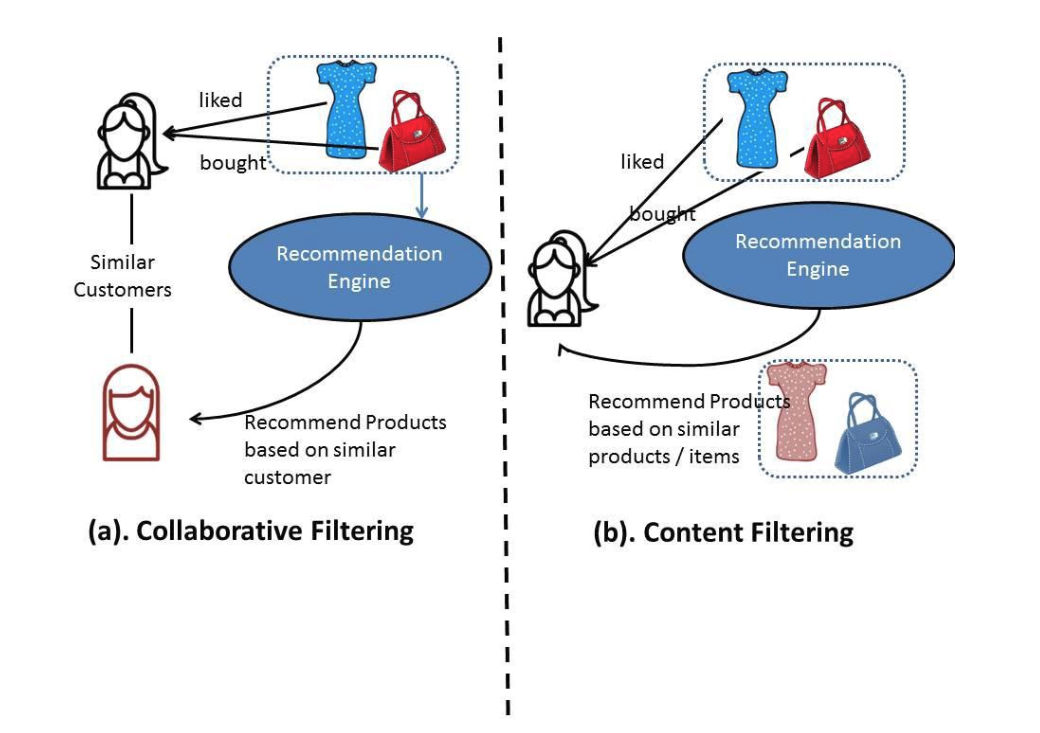
\includegraphics[width=0.9\textwidth]{Figures/recommendationEngine.png}
  \caption[An example of recommendation engine]{An example of recommendation engine\cite{recommendation}}
  \label{fig:recommendation}
\end{figure}

The most common machine learning algorithms are often classified as supervised learning and unsupervised learning.
Supervised learning \cite{supervised} relies on a set of training data which is constructed of various inputs and and correct outputs corresponding to those inputs usually labels. The training data is usually left unchanged and when the test data or data taken from the current user is used as input the algorithm attempts to correctly classify the data based on the training data. The disadvantage of supervised learning is if the incoming data is radically different from the test data the probability of classifying the data into the correct label will be similar and sometimes even lower than classifying into the incorrect label. However because the training data exists it can be quite quicker to setup a supervised learning system then an unsupervised.

Unsupervised learning \cite{unsupervised} uses data that is neither classified or labelled. This allows the algorithm to draw its own conclusions about the data as well as discover hidden structures. If some of the data is similar in any way to another piece of data the algorithm tends to group those pieces of data together. Unsupervised learning is generally more complex and can be more accurate since the algorithm might find subtle discrepancies that might be impossible to notice for a human. This however can lead to unpredictable behaviour where there is expected to be two classifications but instead the data is classified into a lot more than two classifications. Unsupervised learning algorithms typically require more training data than supervised in order to detect similarities and come up with labels.

There are also algorithms that use techniques found in both supervised and unsupervised machine learning these are called Semi-supervised \cite{machineLearning0} machine learning these use a much larger amount of unlabelled training data than labelled. These types of algorithms usually tend to be more accurate than supervised and unsupervised alone.

Another interesting suite of machine learning algorithms is classified into Reinforcement Learning \cite{reinforcementLearning}. These algorithms interact with the environment and received rewards or penalties based on the actions carried out within the environment. If the action carried out receives a reward it is likely that the same action will be repeated again. 

%
%
% End of machine learning
%
%

Achieving synchronisation \cite{sync} is an important part of this project. 
Synchronisation is the process of making two or more data storage devices or programs (in the same or different computers) having exactly the same information at a given time.
Synchronisation is common in multi-threaded software where any number of threads can manipulate the same set of data or even wait for a certain thread to finish execution. For example you wouldn't want your parent thread to finish before the child threads as this can lead to data loss and resources being hogged by a zombie thread. Pthread \cite{pthread} is a great API that can be used for handling threads and shared data between those threads. 
Data Synchronisation \cite{datasync} is an on going process of having the same data present on selected servers. Large databases that operate on multiple servers usually use data versioning to keep check on the latest data. MongoDB is one such database \cite{mongo} this is the reason for a delay when you upload a YouTube video (YouTube doesn't use MongoDB this is just an example) it might not be instantly available for other users to watch as it needs to propagate through a number of servers hosting the databases.
Popular websites use data synchronisation for mirroring websites. This allows users to be distributed among relatively identical servers in order to avoid bandwidth bottlenecks as well as increasing availability just in case one server dies users will be redirected to a different mirror seamlessly without interruptions. 
File synchronisation is the method of choice for home backups this is preferable over the traditional backup methods where data is simply dumped onto another hard drive. This process prevents copying identical files which leads to faster transfers and a less chance of errors occurring. My personal favourite file synchronisation tool is Unison \cite{unison}. It is also possible to synchronise folders over the network between two home computes, Unison does this through SSH.
Blockchain \cite{blockChain} the method used for secure crypto ledgers which also relies on synchronisation between peers. Synchronisation for the ethereum crypto currency blockchain can be expressed as follows. "Synchronisation proceeds from head to known block by requesting and fetching block hashes iteratively from young to old (head to root). Based on block hashes, blocks can be requested. Based on the parenthash of a block, independent sections can be linked and a chain established. By checking if a block is found in the block chain the root of the blockpool can be established and the chain can be inserted in the blockchain."
%#######################################################
%                                                   
% check if its ok to just dump stuff from the web.
%
%#######################################################

%
%
% End of sync
%
%






%
%
% Stick these somehwere maybe 
%
%
Machine learning has been known to be used for secure communications although it is not clear if it is used in servers with valuable data. Google's AI successfully created secure algorithms \cite{GoogleAi1} that use inhuman cryptographic schemes making them harder to crack. This technique is called GAN Cryptography \cite{GoogleAi2} for which a research paper can be found.

Currently dynamic encryption is exercised in voip phone calls by a company known as Dencrypt \cite{dencrypt} according to the explanation of their proprietary algorithm they use a wrapper on top of AES-256 which is a chosen algorithm that is discarded when the data transfer is finished.


This project will be compatible with NodeJs because it is one of the fastest growing server platform \cite{NodeJs} that can be easily set up and supports a large amount of modules.

%
%
% Stick these somehwere maybe ^^^^^^^^^^^^^^^^^^^^^^^^^^^^^^^^^
%
%

%
%
% Notes Start
%
%
Position your topic within Computer Science. This activity will aid you in your literature review also. We zoom out to see three levels:

% notice the enumerate structure to create itemized lists
\begin{enumerate}
    \item What is the core topic your project is about? e.g., Mobile app for online voting.
    \item What core area(s) does the project fall under? e.g., Mobile applications, Social Networking, Service Providers. 
    \item What main area(s) of Computer Science does the project fall under? e.g. Software Development, Cloud Computing.
\end{enumerate}

The ACM Computing Classification System (http://www.acm.org/about/class) will aid you in this, use the 2012 categories. Make sure to use figures and illustrations were appropriate. LaTeX will take care of the formatting of these. Do not try to get fancy here, you should concentrate on the content and not the formatting, this is why we are specifying LaTeX.

% Again take note of the structure, simply copy and paste this for future single figures
\begin{figure}[ht]
  \centering
      
\includegraphics[width=0.7\textwidth]{successkid.jpg}
  \caption[A picture of the success kid!]{A picture of the success kid!\cite{Reference1}}
  \label{fig:successkid}
\end{figure}

You can specify the width and label for a figure which allows you to reference the figure and you can attribute a source in the figure caption as is done for figure \ref{fig:successkid}. Make sure you reference all external figures (i.e. figures you did not create yourself). Also use references for all figures e.g. use "... in figure \ref{fig:successkid} ..." NOT "... in the figure above ...".

%\section{Project Scope}
%Project specifics: Background minimum knowledge.

%Imagine you wanted to explain the specifics of your project to a person that knows nothing of Computer Science. You cannot talk about everything (as the idea is not to write a 500+ page report). Remember the reader at this stage can only be assumed to know what you have covered, so identify what are the minimum concepts belonging to the main areas (listed as 3 in the section before) and the core areas (listed as 2 in the section before) that you would need to explain so that the reader is able to understand the specifics of your project and indeed the following section. For example the minimum amount of knowledge about software development, cloud computing, mobile applications, social networking and service providers that are required so as to understand the specifics of a project about a mobile app for an on-line voting system. Here we are making the same trip we did before, but now in the opposite direction. Start zooming in from 3, then to 2 and finally to reach your project 1. Once the reader is finished this section they should be able to understand the proceeding sections (and have context for it within the project).
%
%
% Notes End
%
%

%
%
% Notes 2.2 Start
%
%
\section{A Review of -INSERT THEMATIC AREA-}
The focus of this section is at the heart of the project research phase. You must identify the main sources of information you should be aware of within your chosen area and pay regular attention to so as to strengthen your knowledge in the core topic you are working at. So here you should develop an knowledge of not only your core topic but also about the area of computer science the topic falls under. More specifically you should research the following:
\begin{itemize}
    \item The top 5 International Conferences and Journals most related to your topic. This is crucial, as it represents the main source for keeping you aware of what the state-of-the-art in your topic is.
    \begin{itemize}
        \item In particular it will make you aware of what other projects related to yours have been already done (so that you can compare/position your project w.r.t. these).
        \item What new techniques are being developed, so that you can apply them in your work. e.g. new frameworks for data visualization
    \end{itemize}
    \item The top 3 most recent books/texts related to your topic. There are many free resources from which you may download a relevant text on the topic of your project. Try to either download or borrow 3 recent (no older than 10 years) texts relating to the topic your project is on which you will use throughout the project as reference material and to aid in tackling a number of the technical problems you may encounter. Any PhD/MSc thesis that have published in the last 5 years relating to the topic are also invaluable resources as they will contain a state of the art and references in your project topic. Approach these only after reading/viewing the wikis/Youtube videos you find as a certain level of knowledge will be assumed about the topic.
    \item The top 5 companies/organizations potentially interested in the product you are developing. Finally, this is also crucial, as it forces you extend to purely programmer view of the project to a wider view considering the market, potential stakeholders and niches where your product can become useful. Moreover, Computer Science is a huge topic with loads of different works and roles. If you pick a project in the area you feel passionate about, and you identify what the market in this area is about, then you can drive your future professional career (from the very beginning) towards the path that makes you happier. I know that this does sound as a very technical reason, but I suppose we all agree is probably the most important of all reasons for choosing a particular project focus. 
    \item The top 5 wiki/forums/blogs/Youtube channels most related to your topic. This is crucial to you as well, as it represents a more accessible, personal and less informal way of communication with people working/interested on the same topic as you are. This communication is extremely helpful for improving your skills, solving potential doubts and increase the interest/relevance of the topic/area itself.
\end{itemize}

You should begin your journey of discovery in reverse order to the listing above (which is given in order of academic importance/significance). So when you are researching your topic first look up some TedX talks or youtube tutorials, then research what companies are doing in the area, then get a handful of very good texts on the core topics of your area (anything older than 5 years usually is not helpful here) and finally start reading conference or journal papers (again newer is better here). In particular during this section you may need to use tables to list resources. These are also automatically formatted in latex thus allowing you to concentrate on content. for example table \ref{tab:Mylar}.

\begin{table}[ht]
	\centering
		\begin{tabular}{ c  c  }
		\hline
		\hline
		Parameter & PET \\
		\hline
		Youngs Modulus & 2800-3100MPa \\
		Tensile Strength & 55-75MPa \\
		Glass Temperature & 75$^\circ$C \\
		Density & 1400kg/m$^3$ \\
		Thermal Conductivity & 0.15-0.24Wm$^{-1}$K$^{-1}$ \\
		Linear Expansion Coefficient & $7\times10^-5$ \\
		Relative Dielectric Constant @ 1MHz & 3\\
		Dielectric Breakdown Strength & 17kVmm$^{-1}$\\
		\end{tabular}
	\caption{PET Physical Properties}
	\label{tab:Mylar}
\end{table}

What has been done before in your community w.r.t. your topic? Once you have gotten an understanding of the topic and technologies and have identified the top 5 formal conferences/journals, wiki/forums/blogs/Youtube channels and companies/organizations the next step is to research in depth on them! And here in depth means in depth. Make sure you cite\cite{Reference1} a number of papers \cite{Reference3}, luckily Latex will take care of the ordering of the citations \cite{Reference2} for you.

The aim here is that you find the trends in your topic (3), and more in general in the area in which your topic resides (2) your project falls under and from these trends you develop your initial project question further and begin to get insights into how others have solved/approached similar problems. Think of this section as colouring in your initial idea. Before you approach this section you should read at least 4/5 good literature reviews (a selection of last years projects will be posted on blackboard to aid you but you should find other sources also).

In particular in this section, you must find and analyse at least 5 (ideally around 10) works belonging to, or at least related to, your work. You must describe these works and position your project w.r.t. them (i.e., clearly identify the similarities and differences between your project and each of these works). Also remember if you find that you are detailing topics that you have not introduced already here you need to add something to the earlier Scope section.
%
%
% Notes 2.2 End
%
%

%
%
% Research papers
%
%
To achieve my goal of dynamically encrypting messages between both parties, each party must know the encryption key without explicitly sending that key to each other. For this to have a dynamic effect multiple processes will in this case synchronise which each other and a separate process will take care of swapping keys.

The research papers that will be cited synchronise once therefore I will just have to take what I learned and apply it to multiple instances.

Two identical neural networks that originally have a random generated state. This state is different between the two networks and to achieve synchronisation this state must be the same, this is because when the state is the same it will be essentially the key used to encrypt messages. And all this will be achieved without ever sending the key over the network even in an encrypted form as in public private encryption techniques. 

A tree parity machine is a common method used across all papers in order to achieve this goal figure \ref{fig:treeParityMachine} visualises such a machine.

\begin{figure}[ht]
  \centering
      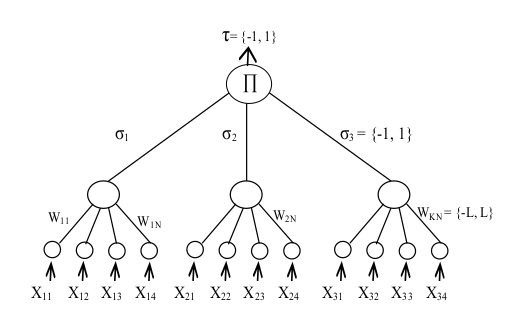
\includegraphics[width=0.7\textwidth]{treeParityMachine.png}
  \caption[Tree parity machine]{Tree parity machine with L=[-4,4], K=3 and N=4\cite{Private_Inputs_to_Tree_Parity_Machine}}
  \label{fig:treeParityMachine}
\end{figure}

According to \cite{Genetic_Key_Guided_Neural_Deep_Learning_based_Encryption} both parties should have the same layout of the tree parity machine where N is the number of neutrons used as input for each hidden neutron. The input neutrons have the X and are at the bottom of the diagram, in this case there are four input neutrons for each hidden neutron. The hidden neutrons are referenced as K, these are the neutrons in the middle with the W in the diagram. These are the weights which are updated if the output of both of the tree parity machines are the same. These weights in the end will be the key used for symmetric encryption between the two parties. T will be the output value which will be compared to the other tree parity machine. 

There is a low number of machine learning algorithms that can be used to synchronise and the paper \cite{Genetic_Key_Guided_Neural_Deep_Learning_based_Encryption} as well as the majority of papers use the hebbian-learning rule figure \ref{fig:hebianFormula}

\begin{figure}[ht]
  \centering
      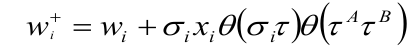
\includegraphics[width=0.7\textwidth]{hebbian_learning.png}
  \caption[Hebbian learning rule]{Hebbian learning rule\cite{Genetic_Key_Guided_Neural_Deep_Learning_based_Encryption}}
  \label{fig:hebianFormula}
\end{figure}

The other two learning rules that can easily be substituted according to this paper \cite{DESIGN_OF_AN_EFFICIENT_NEURAL_KEY_GENERATION} are as follows anti-hebbian learning rule figure \ref{fig:antihebbianlearning} and random-walk rule figure \ref{fig:randomwalklearning}.

\begin{figure}[ht]
  \centering
      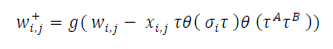
\includegraphics[width=0.7\textwidth]{anti-hebbian.png}
  \caption[Anti-Hebbian learning rule formula]{Anti-Hebbian learning rule formula\cite{DESIGN_OF_AN_EFFICIENT_NEURAL_KEY_GENERATION}}
  \label{fig:antihebbianlearning}
\end{figure}

\begin{figure}[ht]
  \centering
      
\includegraphics[width=0.7\textwidth]{random-walk.png}
  \caption[Random-Walk learning rule formula]{Random-Walk learning rule formula\cite{DESIGN_OF_AN_EFFICIENT_NEURAL_KEY_GENERATION}}
  \label{fig:randomwalklearning}
\end{figure}

There are a number of steps involved in synchronising the tree parity machines.
Step 1. The weights at the beginning should be randomly initialised using local randomisation techniques because there is a chance that downloading data from random APIs can be spoofed which will result in the attacker easily synchronising with your tree parity machine. 

Step 2. Generate random input which will be used by both of the tree parity machines. This input can be generated by a third party server or one of the two parties.

Step 3. Calculate the value of the weights based on the random input using the formula in figure \ref{fig:hiddenNeutronFormula}

\begin{figure}[ht]
  \centering
      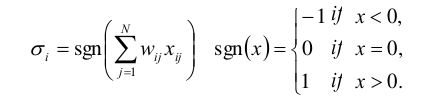
\includegraphics[width=0.7\textwidth]{hidden_neutron_folmula.png}
  \caption[Hidden neutron formula]{Hidden neutron formula\cite{Genetic_Key_Guided_Neural_Deep_Learning_based_Encryption}}
  \label{fig:hiddenNeutronFormula}
\end{figure}

Step 4. Calculate the output neutron based on the weights using the formula in figure \ref{fig:outputNeutronFormula}

\begin{figure}[ht]
  \centering
      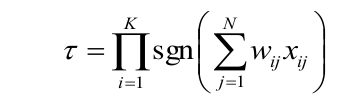
\includegraphics[width=0.7\textwidth]{outputNeutronFormula.png}
  \caption[Output Neutron Formula]{Output Neutron Formula\cite{Genetic_Key_Guided_Neural_Deep_Learning_based_Encryption}}
  \label{fig:outputNeutronFormula}
\end{figure}

Step 5. exchange the output between both of the tree parity machines through a network and if the outputs are not the same repeat again from step 2. And if the outputs are the same apply the hebbian learning rule to the weights and update them accordingly. Repeat step 3 to step 5 until both of the tree parity machines have the same weights.

This technique can be considered too simplistic and the attacker has a greater probability in synchronising with the two parties. I will cover attacks related to tree parity machines further in the section.

To increase the speed of synchronisation and lower the chance of the attacker being able to synchronise with the parties. A technique called queries is used \cite{Private_Inputs_to_Tree_Parity_Machine}.
This technique replaces step 2 from before where the input would be randomly generated by a third party or one of the party. A query consists of a generated vector based on a field of the weights. These queries are then sent from each party to the other interchangeably. 
To calculate the new local field value the following formula can be used figure \ref{fig:LocalFieldFormula}
\begin{figure}[ht]
  \centering
      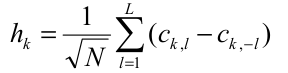
\includegraphics[width=0.7\textwidth]{syncQueriesLocalField.png}
  \caption[Local Field Formula]{Local Field Formula\cite{Private_Inputs_to_Tree_Parity_Machine}}
  \label{fig:LocalFieldFormula}
\end{figure}

It is possible to use a different algorithm where the output \[\sigma_k \] is chosen random for the hidden unit.
It is possible to use the following formula to calculate the local field value. \[ h_k = \sigma_k H \]

To calculate the list of c values that will be used to affect the generation of input values it is possible to use the following two formulas. 
\begin{figure}[ht]
  \centering
      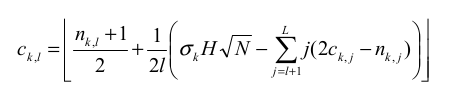
\includegraphics[width=0.7\textwidth]{cformulaa.png}
  \caption[C Formula one]{C Formula one\cite{Private_Inputs_to_Tree_Parity_Machine}}
  \label{fig:LocalFieldFormula}
\end{figure}
\begin{figure}[ht]
  \centering
      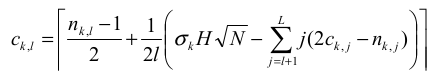
\includegraphics[width=0.7\textwidth]{cformulab.png}
  \caption[C Formula two]{C Formula two\cite{Private_Inputs_to_Tree_Parity_Machine}}
  \label{fig:LocalFieldFormula}
\end{figure}

Where one formula is chosen randomly in each calculation. The probability of one formula being chosen is 50 percent.
Th inputs are then generated and if the inputs are associated with zero weights then the inputs are randomly generated since they do not influence the local field value. 
The input is then divided into L groups and are selected randomly and assigned to \[x_k,_j = sgn(W_k_j) \]
% this double subscript error is fine displays as it should
Finally the remaining input values are set to  \[x_k,_j = -sgn(W_k,_j) \]
To achieve secure key exchange with queries the parties should choose the parameter H so that they can synchronise quickly while the attacker would not be able to do so in time.
Despite the queries being based on the weights an attacker cannot predict the query generated by either party since the weights are never shared. Therefore an attacker can collect the queries but won't be able to establish a mathematical connection between them.
After the synchronisation is complete the weights can be used as a seed for a random generator. As the attacker doesn't know this seed the output of this generator won't be predicted.

There are a number of different attacks that can be carried out on the tree parity machines. These attacks are  more successful if using the basic synchronisation method without the use of queries. This is because up to this date there is no documented or rumoured methods of being able to synchronise with parties who are using queries.

The most basic and useless attack would be a brute force.
This involves trying every possible values for the weights. If using a tree parity machine consisting of 3 hidden neurons, 300 input neurons and 3 weights will result \cite{Private_Inputs_to_Tree_Parity_Machine} in \[3*10^2^5^3\] possible values for the weights making this attack quite impossible using modern computing power. 

The attacker can attempt to learn the weights by using their own tree parity machine with the same number of hidden neutrons and inputs \cite{Private_Inputs_to_Tree_Parity_Machine}. This is essentially identical to the parties tree parity machines but with different initial weights and the attacker synchronises indirectly.
There are three possible situations that can occur with this attack. In these situations A and B will be the two parties trying to synchronise and E is the attacker.
situation 1. Output of A doesn't match output of B and therefore none of the parties including the attacker update their weights.
situation 2. Output of A matches output of B and output of E is also the same. This time A, B and E update their weights.
situation 3. Output of A matches output of B but output of E doesn't match. parties A and B update their weights but E cannot do that and therefore it will take E more time to synchronise to A than it would for B to synchronise with A. Because the learning is ceased after A and B are synchronised E will be left in the dark and not synchronised state. You can further decrease the success rate of this attack by increasing the synaptic depth of the neural network \cite{Private_Inputs_to_Tree_Parity_Machine}. Increasing this will have a performance impact on the parties polynomially however the chance of successful attack decreases exponentially.

More sophisticated attacks can be found in this research paper \cite{BIG_ResearchPaper} such as the genetic attack.
This uses a form of genetic algorithm the key to a successful attack using this method revolves around E being able to determine the fitness of her neural networks.
The attacker spawns a number of tree parity machines which attempt to synchronise with A. After a set time period a selection is made where the most successful synchronised tree parity machines are used to generate the next population. This selection works best if there are certain observable differences between attractive and repulsive effects. 
This attack can be quite successful if the synaptic depth of the neural network is not too large. This can be expressed with the following formula in figure \ref{fig:geneticESuccess} where the probability of E being successful decreases exponentially with the synaptic depth L.
\begin{figure}[ht]
  \centering
      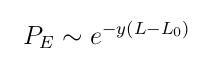
\includegraphics[width=0.3\textwidth]{geneticFormula0.png}
  \caption[probability of E being successful]{probability of E being successful\cite{BIG_ResearchPaper}}
  \label{fig:geneticESuccess}
\end{figure}

In order for this attack to be likely successful the number of tree parity machines the attacker will use will need to be exponentially increased with the increase of the synaptic depth see figure \ref{fig:geneticEMachine}.
\begin{figure}[ht]
  \centering
      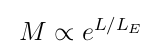
\includegraphics[width=0.3\textwidth]{geneticFormula1.png}
  \caption[Tree Parity Machines needed for synaptic depth]{Tree Parity Machines needed for synaptic depth\cite{BIG_ResearchPaper}}
  \label{fig:geneticEMachine}
\end{figure}
 % Background Theory 

\chapter{Problem - rename to project title}
\label{chap:problem}
\lhead{\emph{Problem Statement}}
The key question to be addressed in this chapter is: "What do I want to achieve".

This chapter should comprise around 1500 words and describe the problem you are trying to solve. Try to be as specific here as you can, this will help you to anticipate possible risks such as lack of support from APIs.

\section{Problem Definition}
Describe the problem you are trying to solve in this project. There will sometimes be a need at some point during the report to display an equation that may be core to your project. For example if the project is on gait detection what equation are you using to determine gait? If the project is on localization what is the method/formula? The formatting of these is reliably done in Latex also as we can see in equation \ref{eq:Legrange}.

\begin{equation}
\frac{d}{dt}(\frac{\partial L}{\partial \dot{c_i}})-\frac{\partial L}{\partial c_i}+\frac{\partial P}{\partial \dot{c_i}} = F_i,
\label{eq:Legrange}
\end{equation}


\section{Objectives}
Enumerate the objectives you want to achieve in your project. Again as this is an early stage these will tend to change but there should be a rational explanation for this change. Always document your work, keep a lab book during the term that you only use for FYP!

\section{Functional Requirements}
Enumerate the functional requirements you want your project to have. 

Please, do not include the use cases here. If you want to create a one-to-one mapping between functional requirements and use cases (which does not necessarily need to be the case, indeed most likely this will not be the case) do it elsewhere. Here should purely describe what do you want to do. In no case should you use this section to provide a description of how to implement them, that is for later. For people doing projects that are not heavy implementation projects (e.g. deploying an architecture or testing a novel tool in specific conditions) this structure can still be used as it will force you to think about what you plan to achieve and what possible metrics you may need to measure success.

Let me explain this with more detail. A common mistake is that people confuse the problem description with the solution approach. This is a common mistake by confusing the \emph{what} with the \emph{how}. Here we are purely focused on the what: What is this project about? What are the objectives? What are the functional and non-functional requirements? 

How are we going to do all these things? Well, this is a question for next chapter. Provided a problem, an objective or a functional requirement, obviously there will usually be many ways of doing it, thus there will be many \emph{hows}, but the definition, the \emph{what} we want to achieve will be unique.

One other display structure you may wish to use at some stage during the report is a figure array. This can also be easily done with Latex and is shown in figure \ref{fig:twosuccesskid}

\begin{figure}
\centering     %%% not \center
\subfigure[Figure A]{\label{fig:a}
\includegraphics[width=0.48\textwidth]{successkid.jpg}}
\subfigure[Figure B]{\label{fig:b}
\includegraphics[width=0.48\textwidth]{successkid.jpg}}
\caption{Two Success kids}
\label{fig:twosuccesskid}
\end{figure}

\section{Non-Functional Requirements}
Enumerate the non-functional requirements you want to achieve in your project (i.e. broadly speaking how your system will operate).

 % Problem

\chapter{Implementation Approach}
\label{chap:implementation}
\lhead{\emph{Implementation Approach}}
The key question to be addressed in this chapter is: "How do I plan to achieve what I have outlined in the previous chapter".

This chapter should comprise around 5000 words and specify your planned implementation approach. Again all sections below are suggestions and will vary significantly from project to project, the key element to be addressed is the core question of the chapter.

\section{Architecture} \label{sec:Arch}
Describe the architecture of the solution that you have in mind, including:
\begin{itemize}
    \item Technologies involved (e.g., frameworks, programming language). 
    \item The hardware needed to develop the project (and to support at deployment stage)
\end{itemize}

Provide a high level view of the system you have in mind, including any package of classes, what is it responsible for and what other packages it communicates to. Provide a high level view of the database (or structure) needed to support the project, including what each table/document is responsible for and the hierarchy among them. You need to be as specific here as you can, why? Because this will aid you in identifying parts of the project you are vague on, this may be fine for some components but cause problems in term 2 for others. If you have hardware element in your project this is also where you provide a high level view of how these elements integrate into the project. So for a project that is cyber-physical you will have both a hardware and software architectural diagram. N.B. This is NOT a full system design but a high level overview of what you can credibly develop. This architecture should be informed by prototyping activity. 

Some of the implementation focused projects may describe how do you envision tackling the functional requirements of your project via a set of use-cases. DFDs are also helpful here to understand elements of your project that may cause problems. You should describe the role of the different parts of the architecture of the solution, and the interaction among them.

\section{Risk Assessment}
Identify any potential risk precluding you from successfully complete your project. This section is really important and often neglected by students resulting in fatal risks occurring in some projects. Make sure to give this section the time it requires. Classify the risk according to their importance, possibility of arising and enumerate the decisions you can make to anticipate them or mitigate them (in case they finally arise). Table \ref{tab:ProjRisks} may help with this classification. This section should include your mitigation approach for any critical risks.

\begin{table}[h]
\centering
\scriptsize
\caption{Initial risk matrix}
\begin{tabular}{|p{2cm}|p{2cm}|p{2cm}| p{2cm} |p{2cm}| p{2cm}|}
\hline \bf Frequency/ Consequence & \bf 1-Rare & \bf 2-Remote & \bf 3-Occasional & \bf 4-Probable & \bf 5-Frequent\\ [10pt]

\hline \bf 4-Fatal & \cellcolor{yellow!50} & \cellcolor{red!50} & \cellcolor{red!50} & \cellcolor{red!50} &\cellcolor{red!50} \\ [10pt]

\hline \bf 3-Critical &\cellcolor{green!50} & \cellcolor{yellow!50} & \cellcolor{yellow!50} & \cellcolor{red!50} &\cellcolor{red!50} \\ [10pt]

\hline \bf 2-Major & \cellcolor{green!50} & \cellcolor{green!50} & \cellcolor{yellow!50} &\cellcolor{yellow!50} &\cellcolor{red!50} \\ [10pt]

\hline \bf 1-Minor & \cellcolor{green!50} & \cellcolor{green!50} & \cellcolor{green!50} &\cellcolor{yellow!50} &\cellcolor{yellow!50} \\ [10pt]
\hline
\end{tabular} \\
\label{tab:ProjRisks}
\end{table}

\section{Methodology}
Describe your personal approach on how to tackle the different parts of this project, including:
\begin{itemize}
    \item How to tackle the needed research to fulfill the background chapter. 
    \item How to set up your Computer Science skills to the project needs (e.g., describe your plan to learn any new technology involved on the project that you are not familiar with). 
    \item What core project managing approach will you follow (e.g., Waterfall, Scrum, etc).
\end{itemize}

\section{Implementation Plan Schedule}
Come up with a schedule for the remaining time (including second semester), so as to describe how do you envision to achieve the implementation of your project by the end of semester 2. This plan SHOULD be ambitious but MUST be realistic and SHOULD be informed by early prototyping and MUST be discussed with your term 1 supervisor.

\section{Evaluation}
Come up with an evaluation plan that allows you to measure how much have you actually achieved the goals of your project. This again is a section that is often neglected where students loose marks. How do you plan to measure the output of your project? A binary it works/does not work is insufficient. You need to be able to quantify the success against both the functional requirements and the initial idea. These are not the same as you may meet all function requirements outlined but not solve the overall problem because you have failed to revisit these and update them with new information which you learn as you are developing the project.

\section{Prototype}
Although you do not have a fully functional project yet, you should show wireframes, snapshots or representation on how do you envision your project to look once the implementation phase has been completed. The nature of this section will vary significantly from project to project and can include anything from code snippets to snapshots of service deployments. Any prototyping you have done during the term should be summarized here that has not been captured in earlier sections. For example if you are planning to host your project using AWS in an EC2 instance you should have at least created a "hello world" setup to determine the basics, this probably should have been discussed in section \ref{sec:Arch}. % Solution Approach

\chapter{Implementation}
\label{chap:imp}
\lhead{\emph{Project Implementation}}
%This chapter should comprise 15 pages and enumerate your experience when doing what you wanted to do the way you wanted to do it.
The implementation of the system has changed drastically since the original plan due to an oversight where it was believed that the Pistache framework could handle the functionality for both the API and the synchronisation between the tree parity machines. The project turned out to be much more involved and difficult than originally expected. This means that the original sprint plan is no longer representative of the actual sprint plan used. This is however to be expected in an agile environment where the following sprint is normally determined after the evaluation of a sprint that was just completed. Despite all of this the system is functional and produces the same outcome as intended.

\section{Difficulties Encountered}
%Enumerate the different difficulties you have found when developing your solution approach. Create three categories of difficulties:
%\begin{itemize}
%    \item \textbf{Easy}: You managed to solve the problem with little difficulty.
%    \item \textbf{Medium}: It was not easy to solve, but you managed to develop a workaround or solution and %still achieve the functionality you originally had in mind.
%    \item \textbf{Hard}: The difficulty was so complicated that you didn’t managed to solve it. As a result, some functional requirement / non-functional requirement or use case from your solution approach was not achieved.
%\end{itemize}

%For each difficulty, classify it into easy, medium or hard. Then, provide the following info:
%\begin{enumerate}
%    \item Description of the difficulty: Brief description of the problem you found.
%    \item How did it affect the original project design?: Indicate how this difficulty affected:
%    \begin{enumerate}
%        \item the architecture of your solution
%        \item if it represented a risk to your project
%        \item if it affected your methodology to develop your project
%        \item if it changed your implementation schedule
%        \item if it changed the evaluation plan
%    \item What did you do to manage the difficulty arisen?: Brief description of your decision to overcome the %difficulty.
%    \end{enumerate}
%\end{enumerate}
The major difficulties I encountered were primarily related to the architecture of the project. The initial class diagrams were way too basic and didn't account for the fact that Pistache would now only be used for the API and nothing else. 

\textbf{Easy Difficulty}
\begin{enumerate}
\item The NodeJs module was replaced with simply a NodeJs App. The NodeJS module is not implemented due to a time constraint and is not necessary to the outcome of the project. The NodeJs module was originally meant to simplify the communication with the API for people who wish to use it. A NodeJS App would need to be implemented regardless in order to use that module and demonstrate the usability of the API. 
The API doesn't have many routes to use therefore it would not be difficult to use the API with any NodeJs App as interacting with the API is simply done with POST requests. The final NodeJs App that is in the same GitHub repository, consumes the API perfectly as well as purposely demonstrating some aspects of dynamic cryptography that would normally be hidden. Any user that wishes to use the API can simply copy the functions in the NodeJs App that interact with the API and change them accordingly to send and receive their own data. It is recommended for users to copy said functions as there are specific steps that need to take place to register the NodeJS App with the API in particular the synchronisation service. For this reason The NodeJs App uses pure NodeJs libraries like ExpressJs \cite{ExpressJS} which is the most popular routing framework for NodeJs. The NodeJs App has no front end as it would be difficult for users wishing to use the API to adapt the front end too, therefore only a basic HTML template engine is used to deal with the HTML. JavaScript for the front end is purely used for visual purposes and is not required since all of the information sent from the browser to the NodeJs app is done through classic HTML forms. This doesn't have any impact on the architecture as the NodeJS App is not really included in the architecture as it is simply designed to consume the API. This does impact the schedule in a positive way as it is easier and quicker to simply make a NodeJS App than a NodeJs module and a NodeJs App.
\end{enumerate}

\textbf{Medium Difficulty}
\begin{enumerate}
\item The sprints needed to be adjusted to accommodate the new implementation plan. The final sprint plan will be placed here as it briefly reflects the major changes that took place, these changes will be discussed in more detail in the following sections. The Sprint plan follows a two week sprint approach.
\begin{table}[h]
\centering
\caption{New Sprint Plan}
\begin{tabular}{|p{1cm}|p{12cm}|}
\hline Sprint & Tasks \\ [14pt]

\hline 1 & Create a basic API server that can process GET and POST requests. Familiarise self with RapidJSON library \cite{rapidjson} and create functions to parse C++ objects into JSON "strings" and JSON "strings" back into C++ objects. Research peer to peer libraries, no useful ones were found. Decided to make a custom one with the help of the Boost ASIO \cite{boost_asio_home} library. Never used Boost ASIO before therefore a decision was made to follow the developers tutorials on the Boost ASIO website. This was not enough to understand the complicated library therefore other tutorials such as this one \cite{boost_asio_totorial_1} were also followed.  \\ [12pt]

\hline 2 & Further knowledge of Boost ASIO needed to be acquired before it was possible proceed with coding the actual peer to peer network. Thankfully a very informative book called Boost.Asio C++ Network Programming \cite{boost_book} by John Torjo was purchased and ended up being the last resource needed in order to complete the peer to peer network. A basic peer to peer network was written however was unstable at the end of this sprint \\ [12pt]

\hline 3 & Peer to peer network works. Implemented basic synchronisation with real tree parity machines. Implemented command line parsing using Boost Program Options \cite{boost_asio_cmd} to enable different options such as selective outputs and port configurations. Completed synchronisation between tree parity machines fully therefore they produce the same weights successfully. Implemented "logging" to external terminal windows. \\ [12pt]

\hline 4 & Research how to proceed with the API i.e have two separate processes or contain the API and peer to peer network within the same process. Decision was made to contain both in the same process for security reasons. Basic API server was constructed and could be easily spawned along side the peer to peer service.\\ [12pt]

\hline 5 & Implement API functionality for synchronisation. Changes needed to be made to the peer to peer service to accommodate unexpected requirements needed to begin synchronisation when using the API. AES encryption decryption implemented using Crypto++ \cite{cryptopp} library. Encrypted data needed to be encoded using base64 again with the help of Crypto++ library. Implement a NodeJs app to consume and demonstrate various features of the API.\\ [12pt]

\hline 5 & Test the system. Implement options to choose which parts of the system to log since logging everything at once can be difficult to demonstrate different aspects of the system. \\ [12pt]

\hline
\end{tabular} \\
\label{tab:ProjRisks}
\end{table}

\FloatBarrier



\item The API and the synchronisation could not be done using only the Pistache framework as originally believed. This was a fairly significant set back since I have experimented before with Pistache framework and was familiar with how it operated functionality wise. It was only until I attempted to use Pistache for synchronisation I discovered that my original plan will not work since Pistache is a very good REST framework and not much else. To synchronise the tree parity machines a peer to peer network seemed most appropriate in how the synchronisation was envisioned to take place. After searching for easy to use libraries that supported peer to peer networks nothing that matched the requirements was found. This lead to the conclusion that a custom peer to peer network would have to be built from scratch. The attention grew towards Boost Asio as it is the most flexible generic networking library for C++. Unfortunately this library is quite extensive and is not as abstract as some of the previous peer to peer libraries encountered. Since with Boost Asio you will still deal with sockets however this will allow for greater control provided you know how the library works and Boost Asio has excellent asynchronous support which is essential for a responsive server. It took almost two full sprints to learn how the library works which set my initial schedule back as it was planned to spend time to learn the new technologies that would be used however it was not expected to spend so much time learning said new technologies. However some of the lost time was made back since the design of the peer to peer network was simple and efficient which allowed for a large number of synchronisation requests to take place per second resulting in generating a valid key in around one second which satisfies the requirement and no further optimisations needed to take place. This occurrence changed the architecture significantly since originally this wasn't meant to be present. Overall I'm glad that this happened as I had a chance to learn one of C++'s most popular networking library. Another benefit of using Boost Asio for synchronisation over Pistache apart from the fact that its impossible to achieve using Pistache is because the Boost Asio library is a lot lighter the performance increase is rather large. Obviously this would be impossible to test fairly however based on Pistache stress tests it can manage roughly 300 - 400 requests per second. The peer to peer Boost Asio can process around one thousand requests per second as it takes around one thousand requests for the tree parity machines to synchronise and they synchronise generally once per second.

\end{enumerate}

\section{Actual Solution Approach}
In December of last year, when writing the first version of the report, in Chapter 4 you came up with your original solution approach. On it, you presented (i) the architecture of your solution, (ii) your list of use cases, (iii) a risk assessment, (iv) a methodology to develop your solution approach, (v) your implementation schedule, (vi) your evaluation plan and (vii) some prototype of the resulting product. From January to April you have been developing your solution approach. Along the way you have encountered difficulties (the ones listed in Section 5.1) which might have modified your original plan so that you can come up with an actual developed project.

This section is effectively the production of "as built" specification where you compare your original design to the final finished project. Please go section by section (the ones listed from (i) to (vii) in the last paragraph. For each section, enumerate any difference between the original design and the final project, and justify the difficulty forcing you to make such this change. Do not fret if some of these changes are radical, what is important here is that there is a clear rationale for changes made. % Conclusions and Term 2 work

%% ----------------------------------------------------------------
\label{Bibliography}
\bibliographystyle{IEEEtranN}  % Use the "IEEE Transaction" BibTeX style for formatting the Bibliography
\bibliography{Bibliography}  % The references (bibliography) information are stored in the file named "Bibliography.bib"
\lhead{\emph{Bibliography}}  % Change the left side page header to "Bibliography"

%% ----------------------------------------------------------------
% Now begin the Appendices, including them as separate files

\addtocontents{toc}{\vspace{2em}} % Add a gap in the Contents, for aesthetics

\appendix % Cue to tell LaTeX that the following 'chapters' are Appendices

\chapter{Code Snippets}

%Put appendix material in this section e.g. code snippets 

%USE THE APPENDICES	% Appendix Title

%\chapter{Wireframe Models} % Appendix Title

%\input{Appendices/AppendixC} % Appendix Title

\addtocontents{toc}{\vspace{2em}}  % Add a gap in the Contents, for aesthetics
\backmatter
\end{document}  % The End
%% ----------------------------------------------------------------